\documentclass{article}\usepackage[]{graphicx}\usepackage[]{xcolor}
% maxwidth is the original width if it is less than linewidth
% otherwise use linewidth (to make sure the graphics do not exceed the margin)
\makeatletter
\def\maxwidth{ %
  \ifdim\Gin@nat@width>\linewidth
    \linewidth
  \else
    \Gin@nat@width
  \fi
}
\makeatother

\definecolor{fgcolor}{rgb}{0.345, 0.345, 0.345}
\newcommand{\hlnum}[1]{\textcolor[rgb]{0.686,0.059,0.569}{#1}}%
\newcommand{\hlsng}[1]{\textcolor[rgb]{0.192,0.494,0.8}{#1}}%
\newcommand{\hlcom}[1]{\textcolor[rgb]{0.678,0.584,0.686}{\textit{#1}}}%
\newcommand{\hlopt}[1]{\textcolor[rgb]{0,0,0}{#1}}%
\newcommand{\hldef}[1]{\textcolor[rgb]{0.345,0.345,0.345}{#1}}%
\newcommand{\hlkwa}[1]{\textcolor[rgb]{0.161,0.373,0.58}{\textbf{#1}}}%
\newcommand{\hlkwb}[1]{\textcolor[rgb]{0.69,0.353,0.396}{#1}}%
\newcommand{\hlkwc}[1]{\textcolor[rgb]{0.333,0.667,0.333}{#1}}%
\newcommand{\hlkwd}[1]{\textcolor[rgb]{0.737,0.353,0.396}{\textbf{#1}}}%
\let\hlipl\hlkwb

\usepackage{framed}
\makeatletter
\newenvironment{kframe}{%
 \def\at@end@of@kframe{}%
 \ifinner\ifhmode%
  \def\at@end@of@kframe{\end{minipage}}%
  \begin{minipage}{\columnwidth}%
 \fi\fi%
 \def\FrameCommand##1{\hskip\@totalleftmargin \hskip-\fboxsep
 \colorbox{shadecolor}{##1}\hskip-\fboxsep
     % There is no \\@totalrightmargin, so:
     \hskip-\linewidth \hskip-\@totalleftmargin \hskip\columnwidth}%
 \MakeFramed {\advance\hsize-\width
   \@totalleftmargin\z@ \linewidth\hsize
   \@setminipage}}%
 {\par\unskip\endMakeFramed%
 \at@end@of@kframe}
\makeatother

\definecolor{shadecolor}{rgb}{.97, .97, .97}
\definecolor{messagecolor}{rgb}{0, 0, 0}
\definecolor{warningcolor}{rgb}{1, 0, 1}
\definecolor{errorcolor}{rgb}{1, 0, 0}
\newenvironment{knitrout}{}{} % an empty environment to be redefined in TeX

\usepackage{alltt}
\usepackage{amsmath} %This allows me to use the align functionality.
                     %If you find yourself trying to replicate
                     %something you found online, ensure you're
                     %loading the necessary packages!
\usepackage{amsfonts}%Math font
\usepackage{graphicx}%For including graphics
\usepackage{hyperref}%For Hyperlinks
\usepackage[shortlabels]{enumitem}% For enumerated lists with labels specified
                                  % We had to run tlmgr_install("enumitem") in R
\hypersetup{colorlinks = true,citecolor=black} %set citations to have black (not green) color
\usepackage{natbib}        %For the bibliography
\setlength{\bibsep}{0pt plus 0.3ex}
\bibliographystyle{apalike}%For the bibliography
\usepackage[margin=0.50in]{geometry}
\usepackage{float}
\usepackage{multicol}

%fix for figures
\usepackage{caption}
\newenvironment{Figure}
  {\par\medskip\noindent\minipage{\linewidth}}
  {\endminipage\par\medskip}
\IfFileExists{upquote.sty}{\usepackage{upquote}}{}
\begin{document}

\vspace{-1in}
\title{Lab 5 -- MATH 240 -- Computational Statistics}

\author{
  Henry Sun \\
  Colgate University  \\
  Department of Mathematics  \\
  {\tt hlsun@colgate.edu}
}

\date{}

\maketitle

\begin{multicols}{2}
\begin{abstract}
This lab aims to answer the question of determining which band: Manchester Orchestra, The Front Bottoms, or All Get Out contributed more to the song ``Allentown." We used Essentia and LIWC to conduct audio and lyrical analysis of song. Manchester Orchestra likely contributed more to the audio, while The Front Bottoms likely contributed more to the lyrics.
\end{abstract}

\noindent \textbf{Keywords:} Installing, loading, and learning to use libraries; working with characters objects; coding \texttt{for()} loops; accessing elements of vectors and lists.

\section{Introduction}
\indent  
In 2018, two bands -- The Front Bottoms and Manchester Orchestra -- released a song they collaborated on called ``Allentown". In a statement to Noisey \citep{vice} -- the music arm of Vice -- Andy Hull of Manchester Orchestra recalled that the creation of this track started when Nate Hussey of All Get Out sent him the first four lines of the track. Andy Hull worked out the melody and music and shared it with Brian Sella of The Front Bottoms, who then helped develop the chorus. 

\indent Throughout this lab, we used Essentia \citep{essentia} to conduct musical analysis on each song, giving us a rough idea of what each band's songs ``sound" like. Using this data, we were able to conclude which band contributed the most to ``Allentown."

\indent In the first week of this lab, we built a batch file (\texttt{batfile.txt}) to process all the song in the directory given to us. We then extracted data from the .JSON Essentia Output, Au Revoir (Adios) in the Talon of the Hawk album by the Front Bottoms, and conducted some musical analysis on the song. 

\indent In the second week of this lab, we continued to compile data for each song from their .JSON file, but we also compiled data from the \texttt{EssentiaModelOutput.csv}, providing us with audio info, and \texttt{LIWCOutput.csv}, providing us with lyrical info. We merge all of the data into a data frame, and used it to create a \texttt{.csv} file for testing and training. 
\columnbreak

\indent Finally, we used \texttt{tidyverse} \citep{tidyverse} to write a function that identified key features that would help us conclude which band contributed the most to ``Allentown" with the aid of plots and tables generated by \texttt{tidyverse} and 
\texttt{xtable} \citep{xtable}.
\section{Methods}
\subsection{Week 1}
After obtaining all of the \texttt{.wav} files for each song, we first began by building a batch file for data processing. Using the \texttt{stringr} package \citep{stringr}, we were able to create the command line prompt for each track, before using \verb|writeLines()| to write all the command lines into the batch file.
Our second task was to process the .JSON Output from a sample song, which we accomplished by using the \texttt{jsonlite} package \citep{jsonlite}. Using this, along with the \texttt{stringr} package, we were able to extract key information from the song, like artist, album, and average loudness. We were then able to use this same skeleton to extract information from every song's .JSON output. 

\subsection{Week 2}
Our first task for the second week of this lab was nearly identical to the procedure followed in the second task from the first week, except that we collected data from the Essentia Model Data \citep{essentiamodel}. This provided us with more auditory information on each song. \\ 
\indent Likewise, we used the LIWC-22 program \citep{liwc} to conduct lyrical analysis on each song. We were able to gather data that describes the thoughts, feelings, and personality traits based on the language used. We extracted additional data by averaging values from certain data points. For example, we can get data on valence and arousal by average the data from the DEAM, emo Music, and MuSe datasets. \\ 
\indent We consolidated the data collected in the previous steps using the \verb|merge()| function. We used this data set to create a testing \texttt{.csv} file, containing only the track ``Allentown" and a training \texttt{.csv} file, containing all tracks except ``Allentown."
\subsection{Week 3}
During our final week, we picked out and summarized key features from each band to determine which one contributed the most to ``Allentown." We first began by calculating the upper and lower fences, and the minimum and maximum for each numerical feature. We compared these values to the same features found in the ``Allentown" track, keeping note of all features within range for one band. Using this data, we were able to create graphs and tables using \verb|ggplot()| and \verb|xtable()| to help us better visualize each feature of interest. 
\section{Results}
In order to identify which band contributed the most to the song, we first began by determining which features in ``Allentown" to analyze. A feature was classified as "Within Range" if the numeric value was between the upper and lower fence for the same feature in each band. This was narrowed down even further to $21$ features having only one band in range. A table of all key features (Table \ref{feat.table}) can be found in the appendix. Overall, we can see that there were no key features with only All Get Out being the only band. However, there were $3$ features within range for The Front Bottoms and $18$ for Manchester Orchestra. It's also crucial to note here that $3$ out of the $4$ lyrical features are within range for The Front Bottoms, while all of the audio features were within range for Manchester Orchestra. \\
\indent Below is a box plot (Figure 1) of the only key feature that is within range of The Front Bottoms. \texttt{positivewords} is one of the three lyrical features (out of four total), along with \texttt{OtherP} and \texttt{conj} within range for The Front Bottoms. This should still be taken with a grain of salt, as \texttt{positivewords} only overlaps with the upper fence, and there are still outliers from both the other bands with more positive words than The Front Bottoms. The \texttt{positivewords} for The Front Bottoms is skewed further right, and has a significantly larger IQR than the other two bands. \\

 \begin{figure}[H]
 %This code is evaluated, but not printed
 %warning=FALSE and message=FALSE ensure no text is returned as a by product of
 %printing; this would cause an error in that plot+text is returned instead of
 %just the plot
\begin{knitrout}
\definecolor{shadecolor}{rgb}{0.969, 0.969, 0.969}\color{fgcolor}
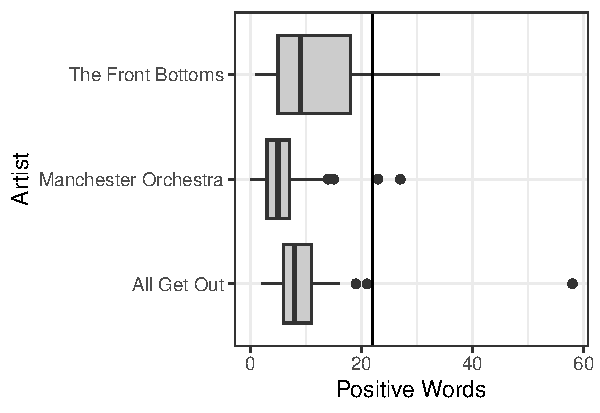
\includegraphics[width=\maxwidth]{figure/unnamed-chunk-1-1} 
\end{knitrout}
 \caption{A boxplot of the \texttt{positivewords} feature for each band. The intercept represents the \texttt{positivewords} value for ``Allentown."}
 \label{plot1} %we can now reference plot1
 \end{figure}
\indent The violin plot below (Figure 2) provides an example of a key feature that is clearly more characteristic of one band. The \verb|average_loudness| of ``Allentown" is within the IQR of Manchester Orchestra, while lying completely out of the upper and lower fence the other bands. However, it is still key to note that the average loudness has a higher variability in Manchester Orchestra compared to the other two bands, which is characterized by its large IQR. \\
\begin{figure}[H]
 %This code is evaluated, but not printed
 %warning=FALSE and message=FALSE ensure no text is returned as a by product of
 %printing; this would cause an error in that plot+text is returned instead of
 %just the plot
\begin{knitrout}
\definecolor{shadecolor}{rgb}{0.969, 0.969, 0.969}\color{fgcolor}
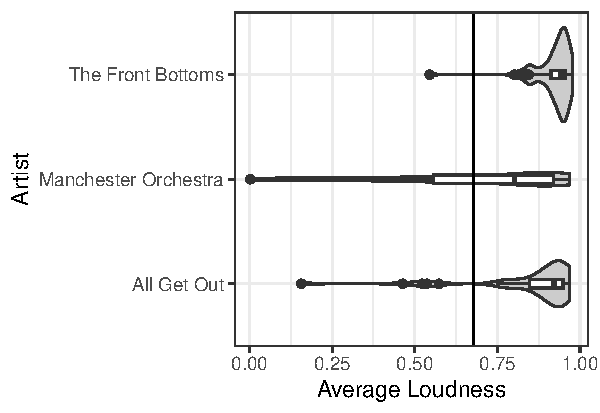
\includegraphics[width=\maxwidth]{figure/unnamed-chunk-2-1} 
\end{knitrout}
 \caption{A violin plot of the average loudness for each band. The intercept represents the average loudness for ``Allentown"}
 \label{plot2} %we can now reference plot1
 \end{figure}
\section{Discussion}
\indent Overall, the analysis of key features in ``Allentown" suggest that Manchester Orchestra had the most significant contribution to ``Allentown" compared to The Front Bottoms and All Get Out. Additionally, there is significant evidence that a lot of the audio features are similar to songs by Manchester Orchestra. To a lesser extent, The Front Bottoms seem to have a larger contribution to the lyrical features of the song, with All Get Out contributing very minimally to the song. \\
\indent This matches up pretty closely to the description of how the song was created in the introduction. The first four lines of the track were created by All Get Out, while the rest of the melody and music was finished by Manchester Orchestra, matching up with Manchester Orchestra's contribution to the audio features. Meanwhile, The Front Bottoms developed the chorus, which matches up with the limited contribution to some lyrical features. \\
\indent Throughout this lab, we've learned how to process and analyze audio and lyrical data, in order to determine the contribution of one artist in a collaborative song or album. This lab has showed us that it's key to make a distinction between audio and lyrical data during analysis. The analysis of data can be quite subjective, as there are numerous ways to filter out data and create tables or plots, which may yield different conclusions.
\pagebreak

%%%%%%%%%%%%%%%%%%%%%%%%%%%%%%%%%%%%%%%%%%%%%%%%%%%%%%%%%%%%%%%%%%%%%%%%%%%%%%%%
% Bibliography
%%%%%%%%%%%%%%%%%%%%%%%%%%%%%%%%%%%%%%%%%%%%%%%%%%%%%%%%%%%%%%%%%%%%%%%%%%%%%%%%
\vspace{2em}

\begin{tiny}
\bibliography{bib}
\end{tiny}
\end{multicols}

%%%%%%%%%%%%%%%%%%%%%%%%%%%%%%%%%%%%%%%%%%%%%%%%%%%%%%%%%%%%%%%%%%%%%%%%%%%%%%%%
% Appendix
%%%%%%%%%%%%%%%%%%%%%%%%%%%%%%%%%%%%%%%%%%%%%%%%%%%%%%%%%%%%%%%%%%%%%%%%%%%%%%%%
\newpage
\onecolumn
\section{Appendix}
\begin{table}[ht]
\centering
\begin{tabular}{rllll}
  \hline
  Key Features & All Get Out & Manchester Orchestra & The Front Bottoms \\ 
  \hline
  spectral\_skewness & Outlying & Within Range & Out of Range \\ 
  spectral\_rolloff & Out of Range & Within Range & Out of Range \\ 
  spectral\_kurtosis & Outlying & Within Range & Out of Range \\ 
  spectral\_entropy & Outlying & Within Range & Out of Range \\ 
  spectral\_energyband\_middle\_high & Out of Range & Within Range & Out of Range \\ 
  spectral\_complexity & Out of Range & Within Range & Out of Range \\ 
  spectral\_centroid & Out of Range & Within Range & Out of Range \\ 
  melbands\_spread & Out of Range & Within Range & Out of Range \\ 
  melbands\_flatness\_db & Out of Range & Within Range & Out of Range \\ 
  erbbands\_skewness & Out of Range & Within Range & Out of Range \\ 
  erbbands\_flatness\_db & Outlying & Within Range & Out of Range \\ 
  dissonance & Outlying & Within Range & Out of Range \\ 
  barkbands\_skewness & Out of Range & Within Range & Out of Range \\ 
  barkbands\_kurtosis & Out of Range & Within Range & Out of Range \\ 
  barkbands\_flatness\_db & Outlying & Within Range & Out of Range \\ 
  average\_loudness & Outlying & Within Range & Outlying \\ 
  chords\_strength & Outlying & Within Range & Out of Range \\ 
  conj & Out of Range & Outlying & Within Range \\ 
  Perception & Out of Range & Within Range & Out of Range \\ 
  OtherP & Outlying & Outlying & Within Range \\ 
  positivewords & Outlying & Outlying & Within Range \\ 
   \hline
\end{tabular}
\caption{A summary of all key features (features only within range for one band)}
\label{feat.table}
\end{table}
\end{document}
